\chapter[Overlays, Groups, Superpositions, and Multipass]
{Control Elements: Overlays, Groups, Superpositions, and Multipass}
\label{c:control}
\index{element!control}
\index{element!lord}
\index{element!slave}

\index{tracking part}
It is possible to have elements controlling the attributes of other
elements. These \vn{lord} elements are meant, for example, to mimic
the effect of changing a knob in the control room. For this purpose
the lattice is split into two sections: The first section is the list
of elements that \bmad uses for any analysis (tracking, Twiss
parameter calculations, etc.). This first part is called the
\vn{tracking} part of the lattice.
Elements in the \vn{tracking} part are either
\vn{slave} elements if they have a controlling lord or \vn{free}
elements if they do not. The second section consists solely of
\vn{lord} elements. \vn{Lord} elements can control other \vn{lord}
elements and a hierarchy of \vn{lord} elements may be established.

There are five types of lord elements: 
\begin{Itemize}
\item 
\index{group}
\vn{Group} lord elements are used to make variations in
attributes. For example, to simulate the action of a control room knob
that changes the beam tune in a storage ring, a \vn{Group} can be used
to vary the strength of selected quads in a specified
manner. \vn{Groups} are covered in \sref{s:group}.
\item
\index{overlay}
An \vn{Overlay} lord is like a \vn{group} except that \vn{overlays}
set the value (not a change in) the attributes they
control. \vn{Overlays} are covered in \sref{s:overlay}.
\item
A \vn{superposition} lord is created when elements are superimposed on
top of other elements. This is covered in \sref{s:super}.
\item
\index{girder}
\vn{Girder} elements mimic the effect of a support girder. This is
covered in \sref{s:girder}.
\item
\index{multipass}
\vn{Multipass} elements are used when the beam recirculates through
the same element multiple times. This is covered in
\sref{s:multipass}.
\end{Itemize}

%-----------------------------------------------------------------------------
\section{Overlay Elements}
\label{s:overlay}

An \vn{overlay} element is used to control the attributes of other elements. 
For example: 
\begin{example}
  over1: overlay = \{a_ele, b_ele:2.0\}, hkick = 0.003
  over2: overlay = \{b_ele\}, hkick
  over2[hkick] = 0.9
  a_ele: quad, hkick = 0.05, ...
  b_ele: rbend, ...
  this_line: line = ( ... a_ele, ... b_ele, ... )
  use, this_line
\end{example}

In the example the overlay \vn{over1} controls the \vn{hkick}
attribute of the "slave" elements \vn{a_ele} and
\vn{b_ele}. \vn{over2} controls the hkick attribute of just
\vn{b_ele}. \vn{over1} has a \vn{hkick} value of 0.003 and \vn{over2}
has been assigned a value for \vn{hkick} of 0.9.

There are coefficients associated with the control of a slave element. 
The default coefficient is 1.0. To specify a coefficient use a vertical colon ":"
after the element name followed by the coefficient. In the above example 
the coefficient for the control of \vn{b_ele} from \vn{over1} is 2.0 
and for the others the default 1.0 is used. thus 
\begin{example}
  a_ele[hkick] = over1[hkick]
               = 0.003
  b_ele[hkick] = over2[hkick] + 2 * over1[hkick] 
               = 0.906
\end{example}
Note: An older notation allowed a slash "/" to be used in place of the
colon ":" for the separator between the slave name and the
coefficient. While the slash is still accepted, its use is
discouraged.

An \vn{overlay} will control all elements of a given name. Thus, in
the above example, if there are multiple elements in \vn{this_line}
with the name \vn{b_ele} then the \vn{over1} and \vn{over2} overlays
will control the hkick attribute of all of them.

Note: Overlays completely determine the value of the attributes that
are controlled by the overlay. in the above example, the hkick of 0.05
assigned directly to \vn{a_ele} is overwritten by the overlay action
of \vn{over1}.

\noindent The default value for an overlay is 0 so for example
\begin{example}
  over3: overlay = \{c_ele\}, k1
\end{example}
will make \vn{c_ele[k1]} = 0. Overlays can also control more than one
type of attribute as the following example shows
\begin{example}
  over4: overlay = \{this_quad[k1]:5.4, this_sextupole[k2], ...\}, hkick
\end{example}


%-----------------------------------------------------------------------------
\section{Group Elements}
\label{s:group}
\index{group}
 
\vn{group} is like \vn{overlay} in that a \vn{group} element controls
the attribute values of other ``slave'' elements. A \vn{group}
element is used to make changes in value. This is unlike an
\vn{overlay} which sets a specific value directly. An example will
make this clear
\begin{example}
  gr: group = \{q1\}, k1 
  gr[command] = 0.34 
  q1, quad, l = ...
  q1[k1] = 0.57
\end{example}
In this example the group \vn{gr} controls the \vn{k1} attribute of
the element \vn{q1}. Unlike overlays, values are assigned to group
elements using the \vn{command} attribute. When a lattice file is
read in then command values for any groups are always applied
last. This is independent of the order that they appear in the file.
Thus in this example the value of q1[k1] would be $0.91 = 0.57 + 0.34$.
When the changes are made to the slave attributes the value of
\vn{command} is stored in the \vn{group}'s \vn{old_command} attribute.
After the lattice is read in a program can change the \vn{gr[command]}
attribute and this change will be added to the value of
\vn{q1[k1]}. The bookkeeping routine that transfers the change from
\vn{gr[command]} to \vn{q1[k1]} doesn't care what the current value of
\vn{q1[k1]} is. It only knows it has to change it by the change in
\vn{gr[command]}.

\index{accordion_edge}
\index{start_edge}
\index{end_edge}
\index{symmetric_edge}
\index{s_offset}
A \vn{group} can be used to control an elements position and length
using the attributes
\begin{example}
  accordion_edge  ! Element grows or shrinks symmetrically
  start_edge      ! Varies element's starting edge s-position
  end_edge        ! Varies element's ending edge s-position
  symmetric_edge  ! Varies element's overall s-position. Constant length.
  s_offset        ! Similar to symmetric_edge
\end{example}
With \vn{accordion_edge}, \vn{start_edge}, \vn{end_edge}, and
\vn{symmetric_edge} the longitudinal position of an elements edges are
varied. This is done by appropriate control of the element's length
and the lengths of the elements to either side. With \vn{s_offset} the
physical element is offset from its reference position
(\sref{s:offset}) and the elements on either side are untouched.
In all cases the total length of the lattice is kept invariant.

As an example, consider \vn{accordion_edge} which varies the edges of
an element so that the center of the element is fixed but the length
varies. With \vn{accordion_edge} a change of, say, 0.1 in a
\vn{group}'s \vn{command} attribute moves both edges of the element by
0.1 meters so that the length of the element changes by 0.2 meters. To
keep the total lattice length invariant the lengths of the elements to
either side are varied accordingly. For example
\begin{example}
  q10: quad, l = ...
  q11: quad, l = ...
  d1: drift, l = ...
  d2: drift, l = ...
  this_line: line = (... d1, q10, d2, q11, ...)
  gr2: group = \{q10\}, start_edge = 0.1
\end{example}
This last line that defines \vn{gr2} is just a shorthand notation for
\begin{example}
  gr2: group = \{q10\}, start_edge 
  gr2[command] = 0.1
\end{example}
The effect will be to lengthen the length of \vn{q10} and shorten the
length of \vn{d1}.

\index{old_command}
\index{command}
\index{coef}
\index{type}
\index{alias}
\index{descrip}
The full list of attributes of a group are
\begin{example}
  command         
  old_command     
  coef            
  type            ! See section \ref{s:string}
  alias           ! See section \ref{s:string}
  descrip         ! See section \ref{s:string}
\end{example}
The \vn{coef} attribute is not used by any \bmad routine. It is
defined for individual programs to store, say, a needed conversion
factor.

Like \vn{overlay}s, coefficients can be specified for the individual
elements under a \vn{group}'s control and \vn{group}s can control more
than one type of attribute. For example
\begin{example}
  gr3: group = \{q1[k1]:-1.0, q2[tilt], oct1:-2.0\}, k3
  gr3[command] = 2.0
  gr3[old_command] = 1.5
\end{example}
In this example \vn{gr3} controls 3 attributes of 3 different
elements. The change in \vn{gr3} when the lattice is read in is $0.5
= 2.0 - 1.5$. this 0.5 change will change \vn{q1[k1]} by $-0.5 = -1
\times 0.5$, \vn{q2[tilt]} will change by 0.5 and \vn{oct1[k3]} will
change by $-1.0 = -2.0 * 0.5$.

%-----------------------------------------------------------------------------
\section{Superposition}
\label{s:super}
\index{superimpose|hyperbf}

In practice the field at a particular point in the lattice may be due
to more than one physical element. A common example is a quadrupole
inside a solenoid. \bmad has a mechanism to handle some of these
cases using what is called ``superposition''. A simple example shows
how this works:
\begin{example}
  Q: quad, l = 10
  D: drift, l = 10
  S: solenoid, l = 6, superimpose, ref = q, ref_end, offset = -1
  lat: line = (Q, D)
  use, lat
\end{example}
The \vn{superimpose} attribute of element \vn{S} superimposes \vn{S}
over the lattice \vn{(Q, D)}. The placement of \vn{S} is such that the
center of \vn{S} is offset -1~meter from the end of \vn{Q} (more on how
superimposed elements get placed later). The tracking part of the
lattice list (the part that one does tracking through) Looks like:
\begin{example}
        Element   Key         Length  Total     
  1)    Q{\#}1       Quadrupole   6        6
  2)    Q{\B}S       Sol_quad     4       10
  3)    S{\#}1       Solenoid     2       12
  4)    D{\#}2       Drift        8       20
\end{example}
What \bmad has done is to split the original elements \vn{(Q, D)} at
the edges of \vn{S}. The first element in the lattice, \vn{Q\#1}, is
the part of \vn{Q} that is outside of \vn{S}. Since this is only part
of \vn{Q}, \bmad has put a \vn{\#1} in the name so that there will be
no confusion. (\vn{\#} has no special meaning other than the fact
that \bmad uses it for mangling names). The next element, \vn{Q{\B}S},
is the part of \vn{Q} that is inside \vn{S}. \vn{Q{\B}S} is a
combination solenoid/quadrupole element as one could
expect. \vn{S{\#}1} is the part of \vn{S} that is outside \vn{Q} so
this element is just a solenoid. Finally, \vn{D\#2} is the rest of the
drift outside \vn{S}.

\begin{figure}[tb]
\centering 
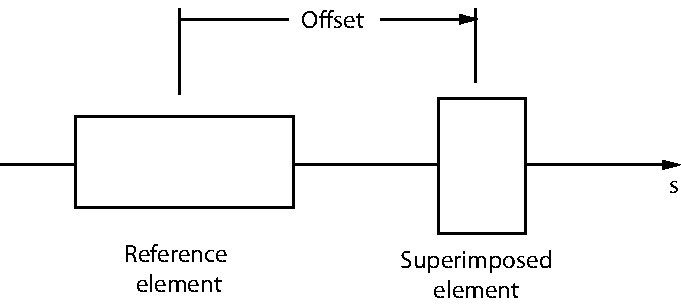
\includegraphics{superimpose.pdf} 
\caption[Superposition Illustration.]
{Illustration of a superposition.}
\label{f:superimpose}
\end{figure}

With the lattice broken up like this \bmad has constructed something
that can be easily analyzed. However, the original elements \vn{Q} and
\vn{S} still exist within the lord section of the lattice. \bmad has
bookkeeping routines so that if a change is made to the \vn{Q} or
\vn{S} elements then these changes can get propagated to the
corresponding slaves. It does not matter which element is
superimposed. Thus, in the above example, \vn{S} could have been put
in the Beam Line (with a drift before it) and \vn{Q} could then have
been superimposed on top and the result would have been the same
(except that the split elements could have different names).

Superpositions are restricted in that \bmad may not have an
appropriate element for the superimposed fields. For example, a
solenoid can not be superimposed over an octupole. If a zero length
element, such as a marker, is superimposed with some other element (or
vice versa) the element is just split in two. For example:
\begin{example}
  Q: quad, l = 10
  M: marker, superimpose, offset = 6
  lat: line = (Q)
  use, lat
\end{example}
The resulting is that the tracking part of the lattice would be
\begin{example}
        Element   Key           Length
  1)    Q{\#}1       Quadrupole    6
  2)    M         Marker        0
  3)    Q{\#}2       Quadrupole    4
\end{example}
and the lord part of the lattice would have the \vn{Q} element.
 
A superposition is illustrated in Figure~\ref{f:superimpose} The
placement of a superimposed element is determined by three factors: A
reference point on the superimposed element, a reference point in the
lattice line, and an offset between the points. The attributes that
determine these three quantities are: 
\index{ref}\index{offset}
\index{ref_beginning}\index{ref_center}\index{ref_end}
\index{ele_beginning}\index{ele_center}\index{ele_end}
\begin{example}
  ref = <element name in lattice>
  offset = <length>      (default = 0)
  ref_beginning
  ref_center             (default)
  ref_end
  ele_beginning
  ele_center             (default)
  ele_end
\end{example}
\vn{ref} sets the reference element. If \vn{ref} is not present then
the start of the lattice is used. \vn{ref_beginning}, \vn{ref_center}
or \vn{ref_end} can be used to indicate where on the reference element
the reference point is. Default is \vn{ref_center}. Similarly,
\vn{ele_beginning}, \vn{ele_center}, or \vn{ele_end} can be used to
indicate the reference point on the superimposed element at the
beginning (entrance) edge, the center, or the end (exit) edge
respectively. If neither of these attributes are given the default is
to use the element center. \vn{offset} is the longitudinal offset
between the reference point on the reference element and the reference
point on the superimposed element. The default if not present is zero.

\index{lattice_type}
\index{linear_lattice}
\index{drift}
\index{overlay}
\index{group}
\index{girder}
Superposition may be done with any element except \vn{Drift},
\vn{Group}, \vn{Overlay}, and \vn{Girder} control elements. A
superimposed element that extends beyond either end of the lattice
will be wrapped around so part of the element will be at the beginning
of the lattice and part of the element will be at the end. For
consistency's sake, this is done even if the \vn{lattice_type} is set
to \vn{linear_lattice} (for example, it is sometimes convenient to
treat a circular lattice as linear). Example:
\begin{example}
  d: drift, l = 10
  q: quad, l = 2, superimpose
  machine: line = (d)
  use, machine
\end{example}
The lattice will have three elements in the tracking section:
\begin{example}
        Element   Key           Length
  3)    Q{\#}2       Quadrupole    1
  2)    D{\#}1       Drift         8
  1)    Q{\#}1       Quadrupole    1
\end{example}
The lord section of the lattice will have the element \vn{Q}. 

When a superposition is made that overlaps a drift the drift, not
being a "real" element, vanishes. That is, it does not get put in the
lord section of the lattice. Thus, it is an error if a second
superposition uses the drift as the reference element. For example
\begin{example}
  dft1: drift, l = 10
  q1: quad, l = 1, superposition, ref = dft1   ! OK 
  q2: quad, l = 2, superposition, ref = dft1   ! ERROR! 
\end{example}
Also note that if aperture limits (\sref{s:limit}) have been assigned
to a drift, the aperture limits can ``disappear'' when the
superposition is done. Explicitly, if the exit end of a drift has been
assigned aperture limits, the limits will disappear if the
superimposed element overlays the exit end of the drift. A similar
situation applies to the entrance end of a drift.

%-----------------------------------------------------------------------------
\subsection{Changing Element Lengths when there is Superposition}
\label{s:super.length}

\index{overlay}
\index{group}
\index{expand_lattice}
When the lattice is constructed, superposition of elements is done
before the addition of any \vn{group} or \vn{overlay} elements. This
is done since \vn{overlay}s and \vn{group}s are allowed to refer
to elements that are superimposed. This can lead to some unexpected
results. For example:
\begin{example}
  q1: quad, l = 10
  q2: quad, l = 10
  lat: line = (q1, q2)
  use, lat
  o: overlay = {q1}, l = 12
  m: marker, superimpose, offset = 15
\end{example} 
In this example, the marker is initially positioned at 15~meters.
The application of the overlay will increase the length of \vn{q1} by
2~meters which will push the marker \vn{m} to 17~meters which is probably 
not what was intended. To avoid this problem, an \vn{expand_lattice} statement
(\sref{s:expand}) can be placed after the overlay, but before the
superimpose, statement
\begin{example}
  ...
  o: overlay = {q1}, l = 12
  expand_lattice
  m: marker, superimpose, offset = 15
\end{example} 

The length of a superimposed element must necessarily be equal to the
sum of the lengths of its slave elements. For example, the element
\vn{S} in the first example of Section~\sref{s:super} has a length of
6~meters which is equal to the sum of the length of \vn{Q{\B}S}
(3~meters) plus the length of \vn{S{\#1}} (also 3~meters).

If a program varies the length of a superimposed element after the
lattice has been parsed, the length of the slaves will be adjusted
accordingly. For example, if element \vn{S} in the first example
of Section~\sref{s:super} is increased from 6~meters to 9~meters, the
lattice would look like
\begin{example}
        Element   Key         Length  Total
  1)    Q{\#}1       Quadrupole   4        4
  2)    Q{\B}S       Sol_quad     6       10
  3)    S{\#}1       Solenoid     3       13
  4)    D{\#}2       Drift        8       21
\end{example}
The length of \vn{Q{\B}S} has been increased from 4~meters to 6~meters
and the length of \vn{S{\#}1} has been increased from 2~meters to
3~meters to give the proper length for \vn{S}. Additionally, to keep
the length of \vn{Q} at 10~meters, the length of \vn{Q{\#}1} has been
decreased to 4~meters. Notice that the overall length of the lattice
has increased by 1~meter. 

Notice that this result is {\em not} what would be obtained if the
length of the element \vn{S} is increased to 9~meters in the lattice
file. The reason for this incompatibility stems from the fact that, in
general, it is a complex problem to have length changes after parsing
mirror what would happen if the lengths were changed in the lattice
file itself. As a result, \bmad chooses to use a relatively simple
algorithm. In practice, lattice layouts can be designed without
superimpose, using the \vn{no_superimpose} command (\sref{s:no.superimpose}), and when the
element lengths are fixed, superposition can be used.


%-----------------------------------------------------------------------------
\section{Multipass}
\label{s:multipass}
\index{multipass|hyperbf}

Some lattices have the beam recirculating through the same element
multiple times. For example, an Energy Recovery Linac (ERL) will
circulate the beam back through the LINAC part to retrieve the energy
in the beam. In \bmad this situation can simulated using the
\vn{multipass} attribute. A simple example shows how this works.
\index{expand_lattice}
\begin{example}
  A: lcavity
  linac_part: line[multipass] = (A, ...)
  my_line: line = (linac_part, ..., linac_part)
  use, my_line
  expand_lattice
  A\B2[dphi0] = 0.5
\end{example}
The tracking part of the lattice consists of two slave elements
\begin{example}
  A\B1, ..., A\B2, ...
\end{example}
Since the two elements are derived from a \vn{multipass} line they are
given unique names by adding a \vn{{\B}n} suffix. In addition there is
a lord element (that doesn't get tracked through) called \vn{A} in the
lord part of the lattice. Changes to attributes of the lord \vn{A}
element will be passed to the slave elements by \bmad's bookkeeping
routines. Assuming \vn{A\B1} is an accelerating cavity, to make
\vn{A\B2} a decelerating cavity the \vn{dphi0} attribute of
\vn{A\B2} is set to 0.5. This is the one attribute that \bmad's
bookkeeping routines will not touch when transferring attribute values
from \vn{A} to its slaves. Notice that the \vn{dphi0} attribute had to
be set after \vn{expand_lattice} (\sref{s:expand})
is used to expand the lattice since
\bmad does immediate evaluation and \vn{A\B2} does not exist before
the lattice is expanded.

Sublines of a multipass line are automatically multipass:
\begin{example}
  a_line: line = (...)
  m_line: line[multipass] = (..., a_line, ...)
\end{example}
In this example \vn{a_line} is implicitly multipass.

Multiple elements of the same name in a multipass line are considered 
physically distinct:
\begin{example}
  m_line: line[multipass] = (A, A, B)
  u_line: line = (m_line, m_line)
  use, u_line
\end{example}
In this example the tracking part of the lattice is
\begin{example}
  A\B1, A\B1, B\B1, A\B2, A\B2, B\B2
\end{example}
In the control section of the lattice there will be two multipass
lords called \vn{A} and one called \vn{B}. The first \vn{A} lord 
controls the 1\St and 4\Th elements in the tracking part of the lattice 
and the second \vn{A} lord controls the 2\Nd and 5\Th elements.

If a multipass line is reversed then the elements are considered to be
transversed backwards:
\begin{example}
  m_line: line[multipass] = (A, A, B)
  u_line: line = (m_line, -m_line)
  use, u_line
\end{example}
In this example the tracking part of the lattice is
\begin{example}
  A\B1, A\B1, B\B1, B\B2, A\B2, A\B2
\end{example}
Here the 1\St and 6\Th elements are connected to a multipass lord and the
2\Nd and 5\Th elements are connected to a different multipass lord.

%-----------------------------------------------------------------------------
\subsection{The Reference Orbit in a Multipass Line}

\index{lcavity}
\index{p0c}\index{e_tot}
If there are \vn{lcavity} elements in the lattice then the reference
energy at a given element may differ from pass to pass. In this case,
the normalized strength (k1, kick, etc.) for magnetic and electric
elements will not be the same from pass to pass. To avoid an
ambiguity, all magnetic and electric elements that are used in a
multipass line must have their magnetic or electric field strength set
as the independent attribute (\sref{s:depend}), {\em or} a reference
energy (\sref{s:energy}) must be defined. A reference energy is
defined by setting \vn{e_tot} or \vn{p0c}, or by setting
\vn{n_ref_pass} as described below. 

\begin{figure}[tb]
\centering 
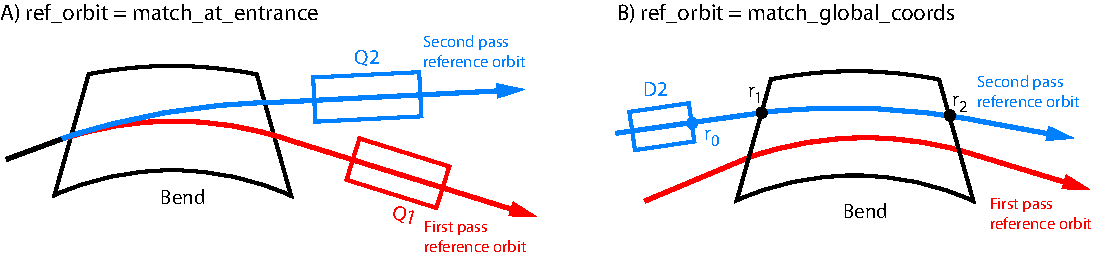
\includegraphics[width=6.2in]{multipass_bend.pdf} 
\caption[The reference orbit with a multipass bend.]  
{A) With \vn{ref_orbit} = \vn{match_at_entrance}, the reference orbits
of different pass will be taken to be the same at the entrance end of
the magnet. If there is a variation of the reference energy through a
bend from pass to pass, the reference orbit through the bend will vary
from pass to pass. B) With \vn{ref_orbit} = \vn{match_global_coords},
the reference orbit on the first pass establishes the position of the
bend in the global coordinate system and the reference orbit on other
passes is calculated with respect to this.}
\label{f:multipass.bend}
\end{figure}

\index{sbend}\index{rbend}\index{patch}
For a bend in a multipass line, there is the added complication of how
to define the reference orbit when the reference energy is different
from pass to pass. If, say, a different reference orbit is used for
each pass there is a problem of how to interpret multipole values
like \vn{k1}. On the other hand, it is sometimes very convenient to be
able to use separate reference orbits. 

A bend element has a \vn{ref_orbit} attribute that, when combined with
the reference energy, define the reference orbit. \vn{ref_orbit} is a
switch that can take the values:
\begin{example}
  single_ref            ! Default. 
  match_global_coords   ! Must be used with n_ref_pass = 1
  match_at_entrance
  match_at_exit
  patch_in              ! Used with patch elements,
  patch_out             !   and must be used with n_ref_pass = 1.
\end{example}
A value of \vn{single_ref} (the default) means that the {\em same}
reference orbit will be used for all passes. The \vn{match_global_coords},
\vn{match_at_entrance} and \vn{match_at_exit} values are used when
{\em separate} reference orbits are desired as described below.

To set the reference energy, one (and only one) of the attributes
\vn{n_ref_pass}, \vn{e_tot} or \vn{p0c} needs to be
set. \vn{n_ref_pass} is an integer indicating which pass is used to
define the reference energy for the lord element. Note: If
\vn{ref_orbit} is set to \vn{match_global_coords}, \vn{n_ref_pass} must be
used and must be set to 1.

An example will make this clear. Consider a bend defined by
\begin{example} 
  B: sbend, l = 1, b_field = 1.0, n_ref_pass = 1, ref_orbit = single_ref
\end{example}
Here the same reference orbit will be used for all passes. Assume that
the reference momentum \vn{p0c} on the first pass is 5~GeV (this is
determined by the reference momentum at the beginning of the lattice
and any \vn{lcavity} elements in the lattice). Since \vn{n_ref_pass}
is one, this fixes the momentum at which the reference orbit is
calculated to be 5~GeV. The bending radius \vn{rho} of the reference
orbit is related to the field and momentum by
\begin{example}
  rho = p0c / (c_light * b_field)
\end{example}
In this case, this translates into a bending radius of 16.7~m. In the
tracking lattice, the first pass element \vn{B\B1} will have a value
for \vn{b_field} of 1~Tesla just like its lord element. Also,
like its lord element, \vn{B\B1} will have an error field,
\vn{b_field_err}, of zero. The total field
\begin{example}
  b_field_tot = b_field + b_field_err
\end{example}
will be 1~Tesla. Additionally, the edge face angles \vn{e1} and
\vn{e2} will be the same as \vn{B}. In this example both are
zero. This is true for all passes.

Now assume that on the second pass, the reference momentum is 10~GeV.
Since, on the second pass, \vn{p0c} is a factor of 2 larger, to keep
the bending radius invariant, the value of \vn{b_field} for the second
pass element \vn{B\B2} will be a factor of 2 larger. That is, it will
be 2~Tesla. However, the total field in the element must be the
same on all passes (\vn{B\B1} and \vn{B\B2} represent the same
physical element after all). Thus, \vn{B\B2} must have a value for
\vn{b_field_err} of -1~Tesla.

Consider the case where the value of
\vn{ref_orbit} is set to \vn{match_at_entrance} and the reference
momentum is set instead of \vn{n_ref_pass}:
\begin{example} 
  B: sbend, l = 1, b_field = 1.0, p0c = 5e9, ref_orbit = match_at_entrance
\end{example}
Here the reference orbit will be different on the two passes. The two
reference orbits will coincide at the entrance edge of the magnet.
This is illustrated in Figure~\ref{f:multipass.bend}A. For both
\vn{B\B1} and \vn{B\B2}, the value of \vn{b_field} will be 1~Tesla
giving bending radii of \vn{16.7}~m and \vn{33.4}~m respectively. With
\vn{B\B2}, the element length will be a slight bit larger than
\vn{B\B1} with a value of \vn{1.0000045}. The entrance face angle
\vn{e1} will always be the same on all passes (zero in this example)
but \vn{e2} will vary. In this case \vn{e2} for \vn{B\B2} will be
\vn{0.003}. With the different reference orbit for the second pass,
there is no good way to handle a non-zero multipole attribute so \bmad
disallows them in this case.

\vn{match_at_exit} is similar to \vn{match_at_entrance} except that
the different reference orbits will coincide at the exit edge of the
magnet. If \vn{match_at_exit} is used with the parameters in the above
example, the only change for \vn{B\B2} is that \vn{e1} will now be
\vn{0.003} and \vn{e2} will be zero.

The \vn{match_at_entrance} value for \vn{ref_orbit} is useful
for simulating a bend at the end of a multipass line that is used to
separate the beams on the various passes. Notice that the next
elements downstream (labeled \vn{Q1} and \vn{Q2} in
Figure~\ref{f:multipass.bend}A) will be physically separated in
space. That is, it does not make sense to use \vn{match_at_entrance}
for a bend that is {\em not} at the end of a multipass
line. Similarly, the \vn{match_at_exit} value is useful for simulating
a bend that combines beams of different energies. Such a bend should
be placed at the beginning of a multipass line.

With \vn{ref_orbit} set to \vn{match_global_coords} the reference
orbit on a given pass is determined by the global coordinates
(\sref{s:global}) of the reference trajectory. Example:
\begin{example} 
  B: sbend, l = 1, b_field = 1.0, n_ref_pass = 1, ref_orbit = match_global_coords
\end{example}
As will be explained, when using \vn{match_global_coords},
\vn{n_ref_pass} must be present and set to 1. With
\vn{match_global_coords}, \vn{B\B1} will have the same parameters as
\vn{B} and this will determine the reference orbit for \vn{B\B1}. See
Figure~\ref{f:multipass.bend}B). For the second pass, the reference
trajectory at the entrance end of the bend is determined as follows:
The calculation starts with the global coordinates of the reference
orbit at the exit end of the element just before \vn{B\B2} (marked
$r_0$ in Figure~\ref{f:multipass.bend}B)). To be physically correct,
this point must lie on the entrance face of \vn{B\B2}. However, it is
possible to have a lattice where this is not so and the calculation
does not demand this. If $r_0$ does not lie on the entrance face, the
reference orbit is extended (either forward or backward) in a straight
line to a point where it intersects the entrance face (marked $r_1$ in
Figure~\ref{f:multipass.bend}B)). The radius of curvature is
calculated by scaling the radius as calculated from the first pass
scaled by the change in reference momentum between the first and
second passes. From the entrance point and the radius of curvature,
the exit point (marked $r_1$ in Figure~\ref{f:multipass.bend}B)) can
be calculated. The curve from $r_1$ to $r_2$ defines the reference
trajectory through \vn{B\B2}. The face angles \vn{e1} and \vn{e2}, and
the path length \vn{l} for \vn{B\B2} can be calculated from the
geometry.

Since the calculation with \vn{match_global_coords} is rather
complicated, the use of \vn{match_global_coords} is restricted to
lattices that lie horizontally in the global $X-Z$ plane. Also, the
restriction to \vn{n_ref_pass = 1} is necessary since the calculation
becomes nondeterministic otherwise. 

Additionally, for a bend, with \vn{ref_orbit} set to
\vn{match_at_entrance}, \vn{match_at_exit} or
\vn{match_global_coords}, the bend must be a pure dipole. That is, no
quadrupole or higher order components. This assumption is
necessary since the reference orbit calculation assumes that the
orbit within the bend is circular for all reference orbits.

%-----------------------------------------------------------------------------
\subsection{Using Patch elements to Vary the Reference Orbit in a Multipass Line}
\label{s:multi.patch}

\begin{figure}[tb]
\centering 
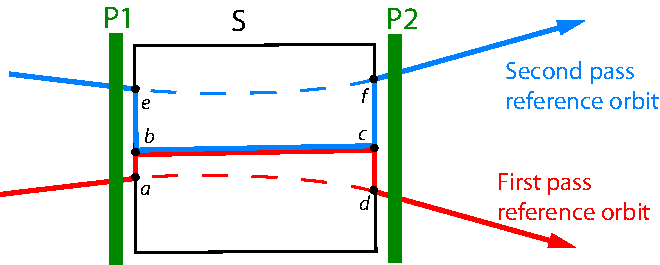
\includegraphics[width=4in]{multipass_patch.pdf} 
\caption[Using patch elements to vary the reference orbit in a multipass line.]
{Using patch elements to vary the reference orbit in a multipass line. 
The gap between \vn{patch} elements \vn{P1} and \vn{P2} and the lattice section 
\vn{S} is for illustration purposes only.
}
\label{f:multipass.patch}
\end{figure}

There exist situations where it is desirable to have a different
reference orbits for each pass through a non-bend elements. Such a
situation is illustrated in Figure~\ref{f:multipass.patch}. In this
example, beams of differing energy pass through an a section of the
lattice labeled \vn{S}. This section may contain one or more
elements. The desired reference orbit for each pass follows the beam
trajectories. This is achieved by placing patch elements, called
\vn{P1} and \vn{P2}, just before and just after \vn{S}. The
corresponding lattice file would look like
\begin{example}
  p1: patch, ref_orbit = patch_in, n_ref_pass = 1, translate_after = True
  p2: patch, ref_orbit = patch_out, n_ref_pass = 1, ref_patch = p1

  m_line: line[multipass] = (p1, S, p2)
  all_line: line = (..., m_line, ..., m_line, ...)
  use, all_line
  
  expand_lattice
  p1\B1[x_offset] = 0.05
  p1\B1[x_pitch] = -0.0034
\end{example}
The \vn{ref_orbit} parameter for \vn{p1} and \vn{p2} indicate whether
the patch is just before (\vn{patch_in}) or just after
(\vn{patch_out}) the section of interest. In this example,
\vn{x_offset} and \vn{x_pitch} parameters for the first pass slave
\vn{p1\B1} are set in the lattice file. This determines the
orientation of the reference orbit through \vn{S} (labeled $b$-$c$ in
the figure) with respect to the incoming first pass reference
orbit. Point $a$ in the figure is the first pass reference orbit just
before \vn{p1\B1} and point $b$ is the reference orbit just after. On
the second pass, \bmad will calculate the patch parameters for
\vn{p1\B2} so that the global coordinates of the reference orbit just
after \vn{p1\B2} is the same as the reference orbit just after
\vn{p1\B1}. That is, point $b$.

The patch parameters for the \vn{p2\B1} first pass slave of \vn{p2},
which has \vn{ref_orbit} set to \vn{patch_out}, the calculation is as
follows: In the definition of \vn{p2} the \vn{ref_patch} parameter is
set to \vn{p1}. \bmad uses this as the starting point for
tracking. \bmad starts with a particle on the reference trajectory
just {\em before} \vn{p1\B1} and tracks it to the end of \vn{S} (curve
$a$-$d$ in the figure). \bmad then sets the parameters of \vn{p2\B1}
so that the reference orbit after the patch (point $d$) coincides
with the particle. The calculation of the second pass slave \vn{p2\B2}
is analogously computed.

The above procedure of defining the reference orbit using patches with
\vn{ref_orbit} set to \vn{patch_in} and \vn{patch_out} is helpful in
designing lattices. However, once a lattice is designed, there will be
a problem for simulations of lattice errors since particle
trajectories, and hence the reference orbit, will be affected by such
errors. To avoid this, once the layout of the lattice has been settled
on, the \vn{patch_in} and \vn{patch_out} patches should be removed and
four new patches, to replace the four multipass slave patches, should
be introduced outside of the multipass section with the patch
parameters set to the appropriate values.
